\chaptermark{Introduction}
\chapter{Introduction}
\label{ch:introduction}
The Greek philosopher Heraclitus once said that one constant since the beginning of time is change. However, the fear of change is also a constant.  His central claim is summed up in the phrase Panta Rhei ("life is flux"), recognising life's essential, underlying essence as change\footnote[1]{\url{https://plato.stanford.edu/entries/process-philosophy/}}. Nothing in life is permanent, nor can it be, because the very nature of existence is change. Since times immemorial\footnote{Reaching beyond the limits of memory, tradition, or recorded history.}, humans have liked routine, making us feel in control of our lives. When that fear of change becomes irrational, our ability to control it becomes a phobia, particularly Metathesiophobia. A Metathesiophobe feels they have no control over their lives due to constant change. Metathesiophobes tend to live in the past and are unwilling to progress, often leading to depression, seriously impacting their professional and personal lives \parencite{PsychTimes}. If a society or country rejects the change, there is no growth and no progress. The inability to change, progress, or grow can result in stagnation. Stagnation rejects realising ones full potential. \parencite{Mark2010, Arapahoe2020}

A world that is continuously in flux is a volatile, uncertain, complex and ambiguous world. \parencite{Bennett2014,Sinha2020} According to \textcite{Bennett2014} the world of \acrfull{vuca} requires a new approach. Disintermediation\footnote{Disintermediation is the process of cutting out one or more middlemen from a transaction, supply chain, or decision-making process.}, globalisation, market upheaval, disruption, and technological advance all combine to produce an effect that is difficult to mitigate,  impossible to predict, and arduous\footnote{Hard to accomplish or achieve.} to detect \parencite[p. 885]{OReilly2019}. \textcite{Taleb2008} his definition of a black swan (see later in this chapter) is similar. To deal with the \acrshort{vuca} world, companies invested a great deal of time and money in becoming less \gls{fragile} by being more \gls{robust} and \gls{resilient}. However, \textcite{Taleb2012} claims that by being more \gls{robust}, or \gls{resilient}, the company can only withstand the change but does not gain from it.

\textcite{Taleb2012} defines the opposite state of \gls{fragile}, \gls{antifragile} as an answer to what \textcite{Taleb2008} calls black swan events. \textcite{Taleb2012} states that \gls{resilient}, \gls{robust} (and company) are states that neither breaks nor improves. \textcite{Taleb2012} claims that \gls{antifragile} is the state that gains and improves. \Gls{antifragile} is the true opposite of \gls{fragile}.

In this thesis, I define the \acrfull{ea} success factors for contribution to become \gls{antifragile}.

\section{The author}
\label{sec:context}
I am working as a Chief Architect for an \acrfull{isv} delivering products and services to the local governmental agencies in The Netherlands, such as municipalities, the local tax offices, and the social services. I am responsible for the architecture function in this company. With architecture we use an outside-in approach. We monitor our external environment, the public sector, and translate this into changes for our organisation, services and products. We do this to stay relevant in the market we serve, the public sector market. Until now we invested a lot in being more resilient and more robust to the changes from our environment but we are still not gaining from it. I want my organisation to gain from all those changes. \Gls{antifragile} can help us to achieve this goal.

\section{The structure of this thesis}
\label{sec:structure}
In \cref{ch:introduction}, the context of the research is set, the core concepts of \acrshort{ea} and \glspl{antifragile} are introduced together with the the public sector. The Chapter states the problem statement, the research questions, and the substantiation of the relevance of the research. In \cref{ch:theoreticalbackground}, the background on the concepts is given. The lens of the public sector is defined. \cref{ch:research-methodology} explains the used research methodology and the approach for the research based on the FAIR\footnote{\url{https://www.go-fair.org/fair-principles/}} principles and the research properties of replicability, falsification, independence, and precision as described by \textcite{Recker2013}. \cref{ch:eaafsuccessfactors} describes the found success factors. Implementation guidelines from an \acrshort{ea} perspective operationalise the found success factors. \cref{ch:eaafsuccessfactors} ends with an overview of found success factors of \acrshort{ea} and \gls{antifragile} that can contribute to the public sector to become \gls{antifragile}. In \cref{ch:delphi} the Delphi method is used to refine, validate, and extend the success factors. The success factors are weighted and screened to determine the concluding set of success factors by triangulation. Finally, the conclusion, discussion and recommendations are in \cref{ch:conclusionanddiscussions}. This thesis ends with \cref{ch:retrospective} for a retrospective on the research and its process.

\section{Introduction of the public sector}
\label{sec:intropublicsector}
According to \textcite{PrivacySense2016} the public sector is comprised of organisations that are owned and operated by the government and exist to provide services for its citizens. Similar to the non-profit sector, organisations in the public sector do not seek to generate a profit. \textcite{PrivacySense2016} divides the public sector into three levels.

\begin{itemize}
	\item{\textbf{The national government,} such as the military, the tax authority, and homeland affairs.}
	\item{\textbf{The regional government,} such as the provinces, the police, and water management.}
	\item{\textbf{The local government,} such as the municipalities, the social services, and the local tax offices.}
\end{itemize}
I use the local government as my lens for the research. The regional and national governments are part of the environment (\cref{sec:introea}).

\section{Introduction of the concept Enterprise Architecture}
\label{sec:introea}

\textcite[p. 104]{Lapalme2016} says that \acrshort{ea} should be understood as being constituted of the essential elements of a socio-technical organisation, their relationships to each other and their changing environment, as well as the principles of the organisation’s design and evolution. Enterprise architecture management is the continuous practice of describing and updating the EA to understand the complexity and manage change. Architects use an \gls{archframework} for describing \acrshort{ea}. Most of the frameworks use a layered approach for specific viewpoints on a system. The most used layers are business, information, applications, and technology. \textcite[p. 189]{Ylimaeki2005} suggests that \acrshort{ea} is an approach for controlling the complexity and constant changes in the business environment of an organisation, enabling alignment between the business vision, business requirements and information systems.

\begin{remark}
based on feedback Edzo. Add some examples to layering (TOGAF, Dieter his framework, etc...)
\end{remark}

\section{Introduction of the concept of antifragility}
\label{sec:introantifragility}
\textcite{Taleb2008} describes a black swan as an event that 1) is so rare that even the possibility that it might occur is unknown, 2) has a catastrophic impact when it does occur, and 3) is explained in hindsight as if it were actually predictable. For extremely rare events, \citeauthor{Taleb2008} argues that the standard tools of probability and prediction, such as the normal distribution, do not apply since they depend on large population and past sample sizes that are never available for rare events by definition. Extrapolating, using statistics based on observations of past events is not helpful for predicting black swans and might even make us more vulnerable to them. In his book \Gls{antifragile}, \textcite{Taleb2012} states that the way to survive a black swan event is to be \gls{antifragile}.

Most people answer that the opposite of \gls{fragile} is \gls{robust}, \gls{resilient}, solid, or something of the sort. However, the \gls{resilient}, \gls{robust} (and company) are items that neither break nor improve, so you would not need to write anything on them — have you ever seen a package with \gls{robust} in thick green letters stamped on it? Logically, the exact opposite of a \gls{fragile} parcel would be a package on which one has written; please mishandle or please handle carelessly. Its contents would not just be unbreakable but would benefit from shocks and a wide array of trauma \parencite{Taleb2012}. \textcite[p. 32]{Botjes2020} mentions that almost all if not all papers on antifragility and resilience use the term stressor for an event from outside the system that causes stress. 

\begin{figure}[h!]
	\centering
	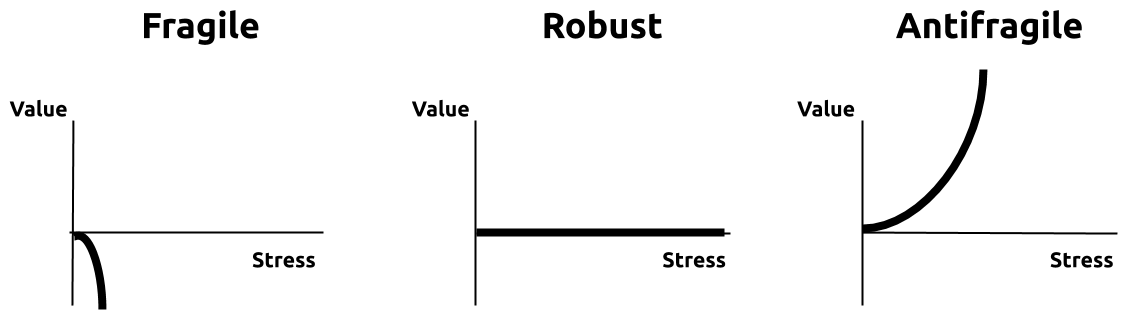
\includegraphics[width=0.7\linewidth]{images/eaal-triad}
	\caption[EAAL Triad]{\acrfull{eaal} Triad \parencite{Botjes2020}}
	\label{fig:eaal-triad}
\end{figure}

\section{Problem statement}
\label{sec:problemstatement}
The concept of \gls{antifragility} implies that organisations could benefit and strengthen from crises, volatility, errors and uncertainty and could also lead to opportunities for innovation \parencite{Kastner2017}. \acrshort{ea} is a discipline that helps organisations to reach their goals. As described in \cref{introea} with \acrshort{ea} one would expect that an organisation uses \acrshort{ea} to get more towards the state of \gls{antifragility}. The already conducted research had its focus on the layers of application and information but not on \acrshort{ea}. The problem is that the \acrlong{bok} contains no direct knowledge on how to achieve \gls{antifragility} with the use of \acrshort{ea}. 

\section{The research subject}
\label{sec:researchsubject}
As described in \cref{sec:introea} \acrshort{ea} is an approach for controlling the complexity and constant changes in the business environment of an organisation, enabling alignment between the business vision, business requirements and information systems. So \acrshort{ea} facilitates an organisation in assessing the impact of change and making recommendations for target states that support business objectives. \acrshort{ea} can help organisations in changing towards the state of \gls{antifragility}.

However, what are the success factors of \acrshort{ea} that contribute to accomplishing \gls{antifragility}? 
\begin{figure}[H]
	\centering
	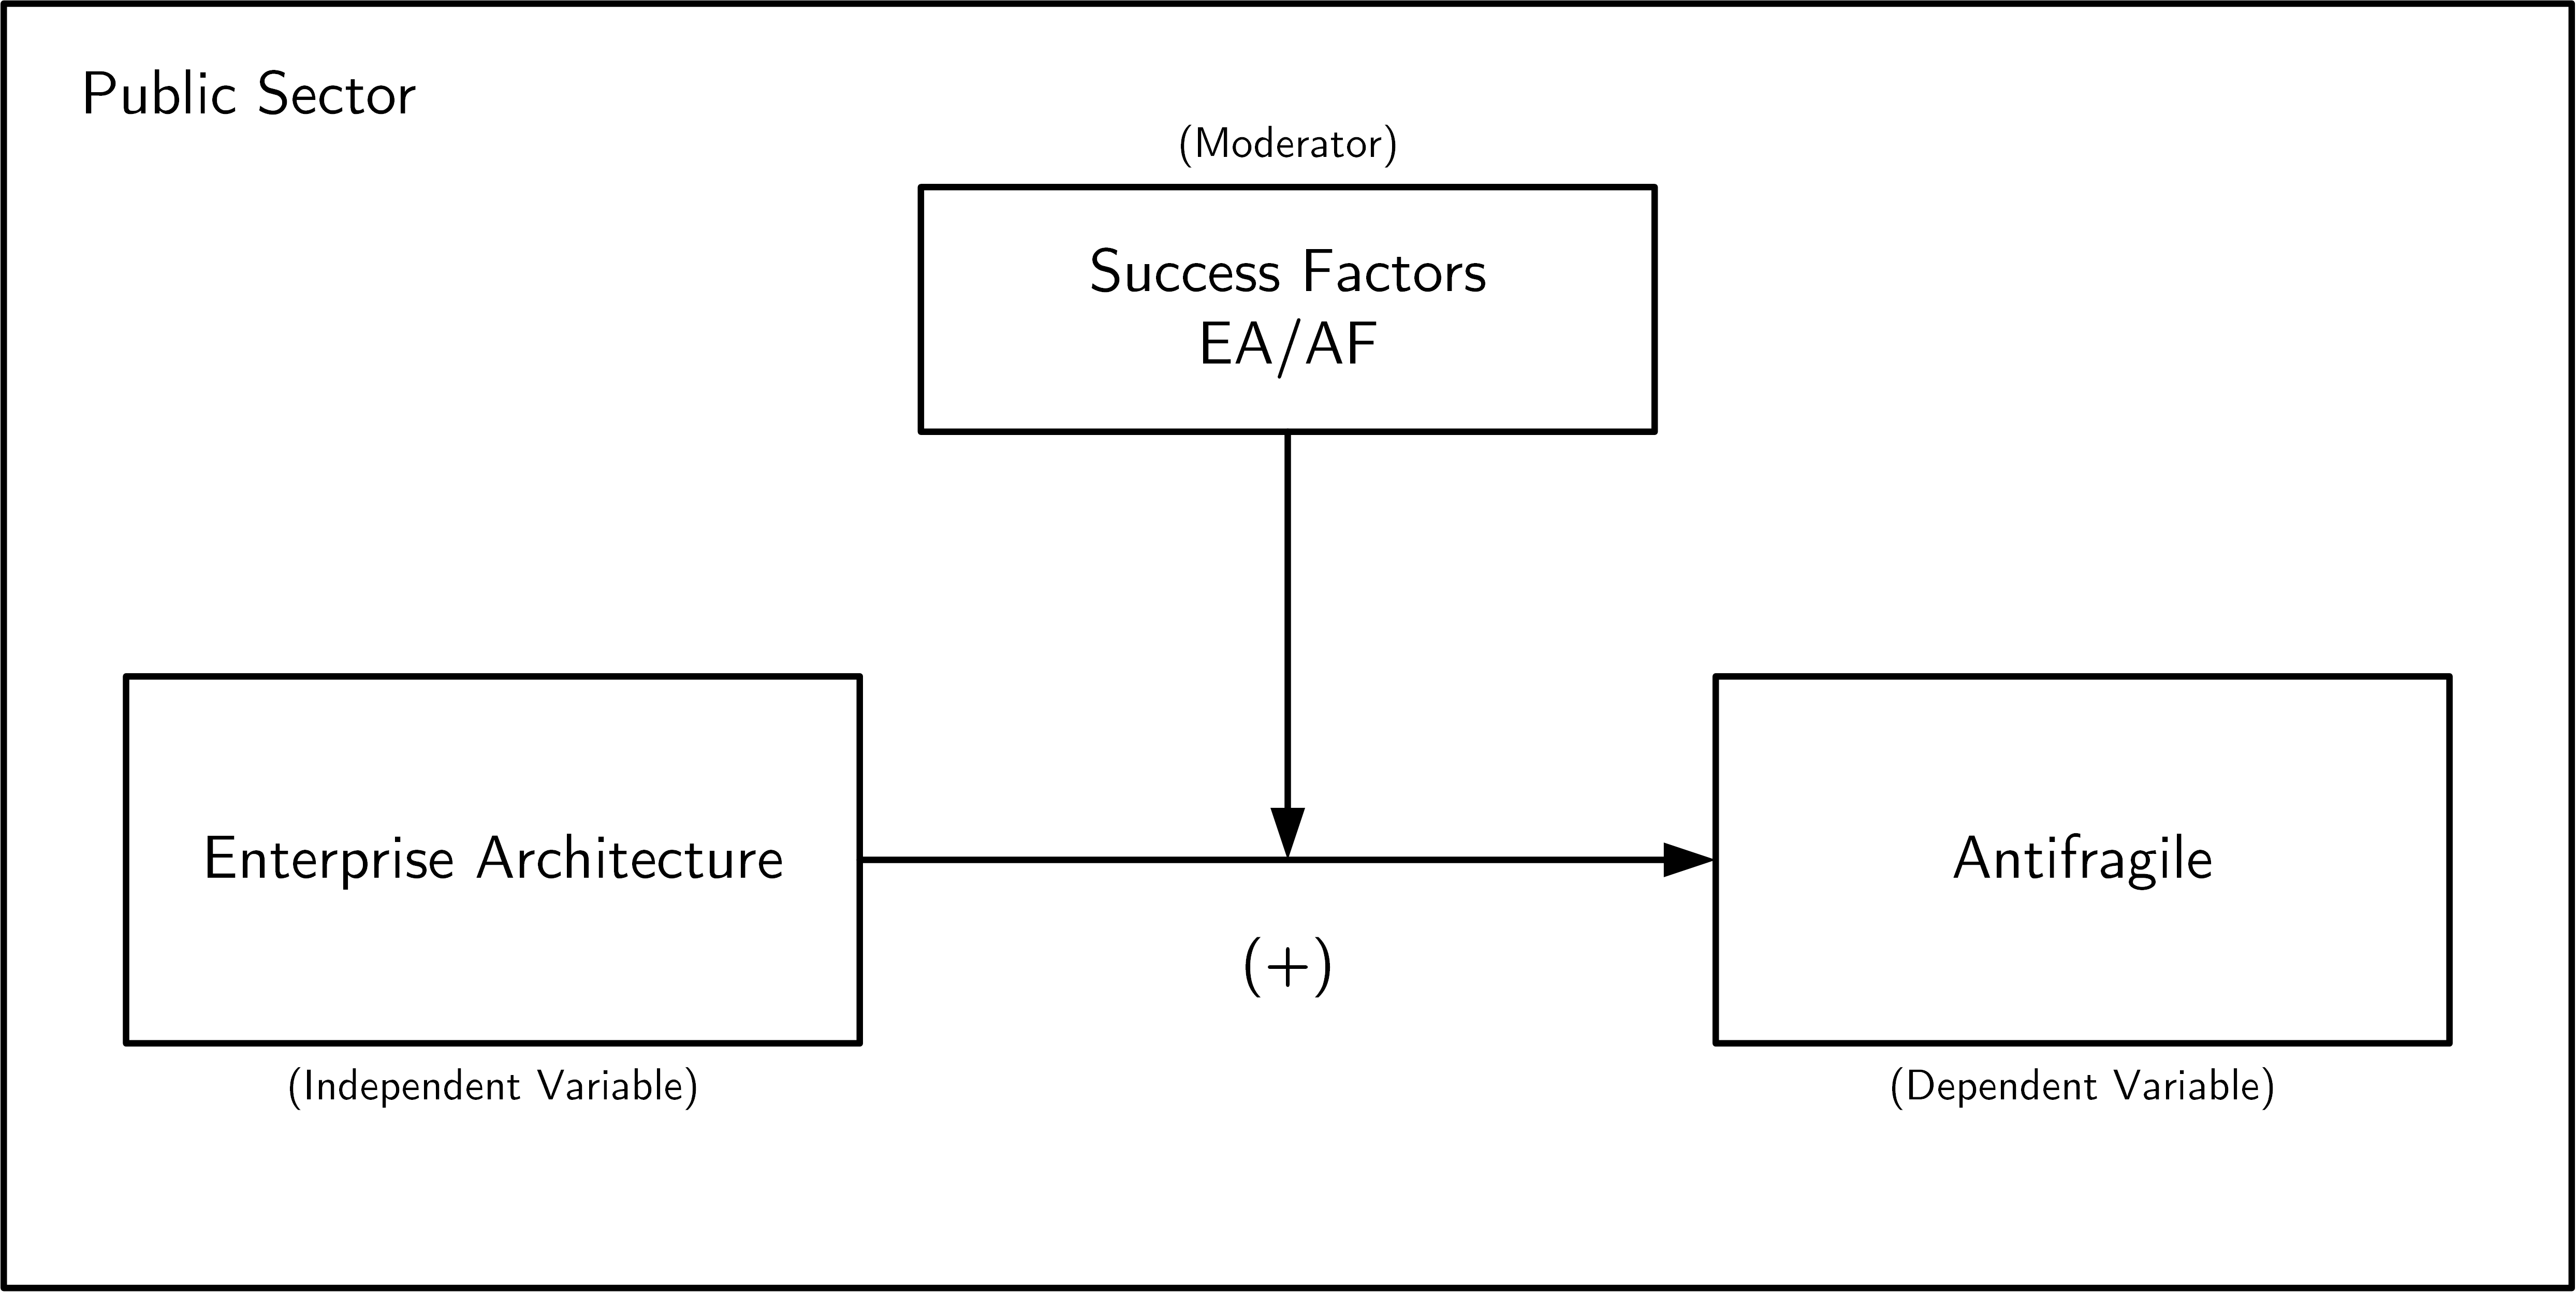
\includegraphics[width=0.8\linewidth]{images/conceptualmodel}
	\caption[Conceptual Research Model]{Conceptual Research Model}
	\label{fig:conceptualmodel}
\end{figure}

The conceptual research model hypothesises that, in the context of the public sector, \acrlong{ea} success factors have a positive influence on the contribution of \acrlong{ea} in achieving antifragility in the public sector. From this conceptual research model, the research question is:\bigskip

\noindent \emph{''What are the success factors of \acrlong{ea} for \gls{antifragility} in the public sector?''}\bigskip

The sub-questions support the research question:

\begin{enumerate}
	\item{What is the literature saying about the public sector?}
	\item{What is the literature saying about \acrlong{ea}?}
	\item{What is the literature saying about the success factors of Enterprise Architecture?}
	\item{What does the literature say about antifragile?}
	\item{How can the success factors of \acrlong{ea} contribute to becoming antifragile?}
\end{enumerate}
\section{Research relevance}
\label{sec:researchrelevance}

\acrshort{ea} has contributed to being more \gls{robust}, \gls{resilient}, and \gls{agile}. Using \acrshort{ea} in pursuing \gls{antifragility} will add value to companies by accelerating and growing when there is a stressor or black swan event. The \gls{antifragile} theory is young.  \citeauthor{Taleb2012} published the theory in his book ''\Gls{antifragile}: Things that gain from disorder.'' in \citeyear{Taleb2012}.  Studies conducted on \acrshort{ea} with the concept of \gls{antifragile} are almost non-existence. The conducted studies are primarily about making IT Systems \gls{antifragile}. \textcite{Botjes2020,Kastner2017} are exceptions and have researched how to apply \gls{antifragile} in an organisational context. Nevertheless, both concluded that there is more research needed. The former used the lens of Enterprise Engineering, which is closely related to \acrshort{ea}, together with complex adaptive system resilience, while the latter used mostly resilience as its lens. There is still no answer to how \acrshort{ea} can contribute to becoming \gls{antifragile}. Giving more insights on this subject will contribute to the \acrshort{bok} and help others get closer to \gls{antifragility} by using \acrshort{ea}.
{\let\thefootnote\relax\footnote{{\url{https://www.istockphoto.com/en/vector/506120634-84046799}}}}
\begin{figure}[H]
	\centering
	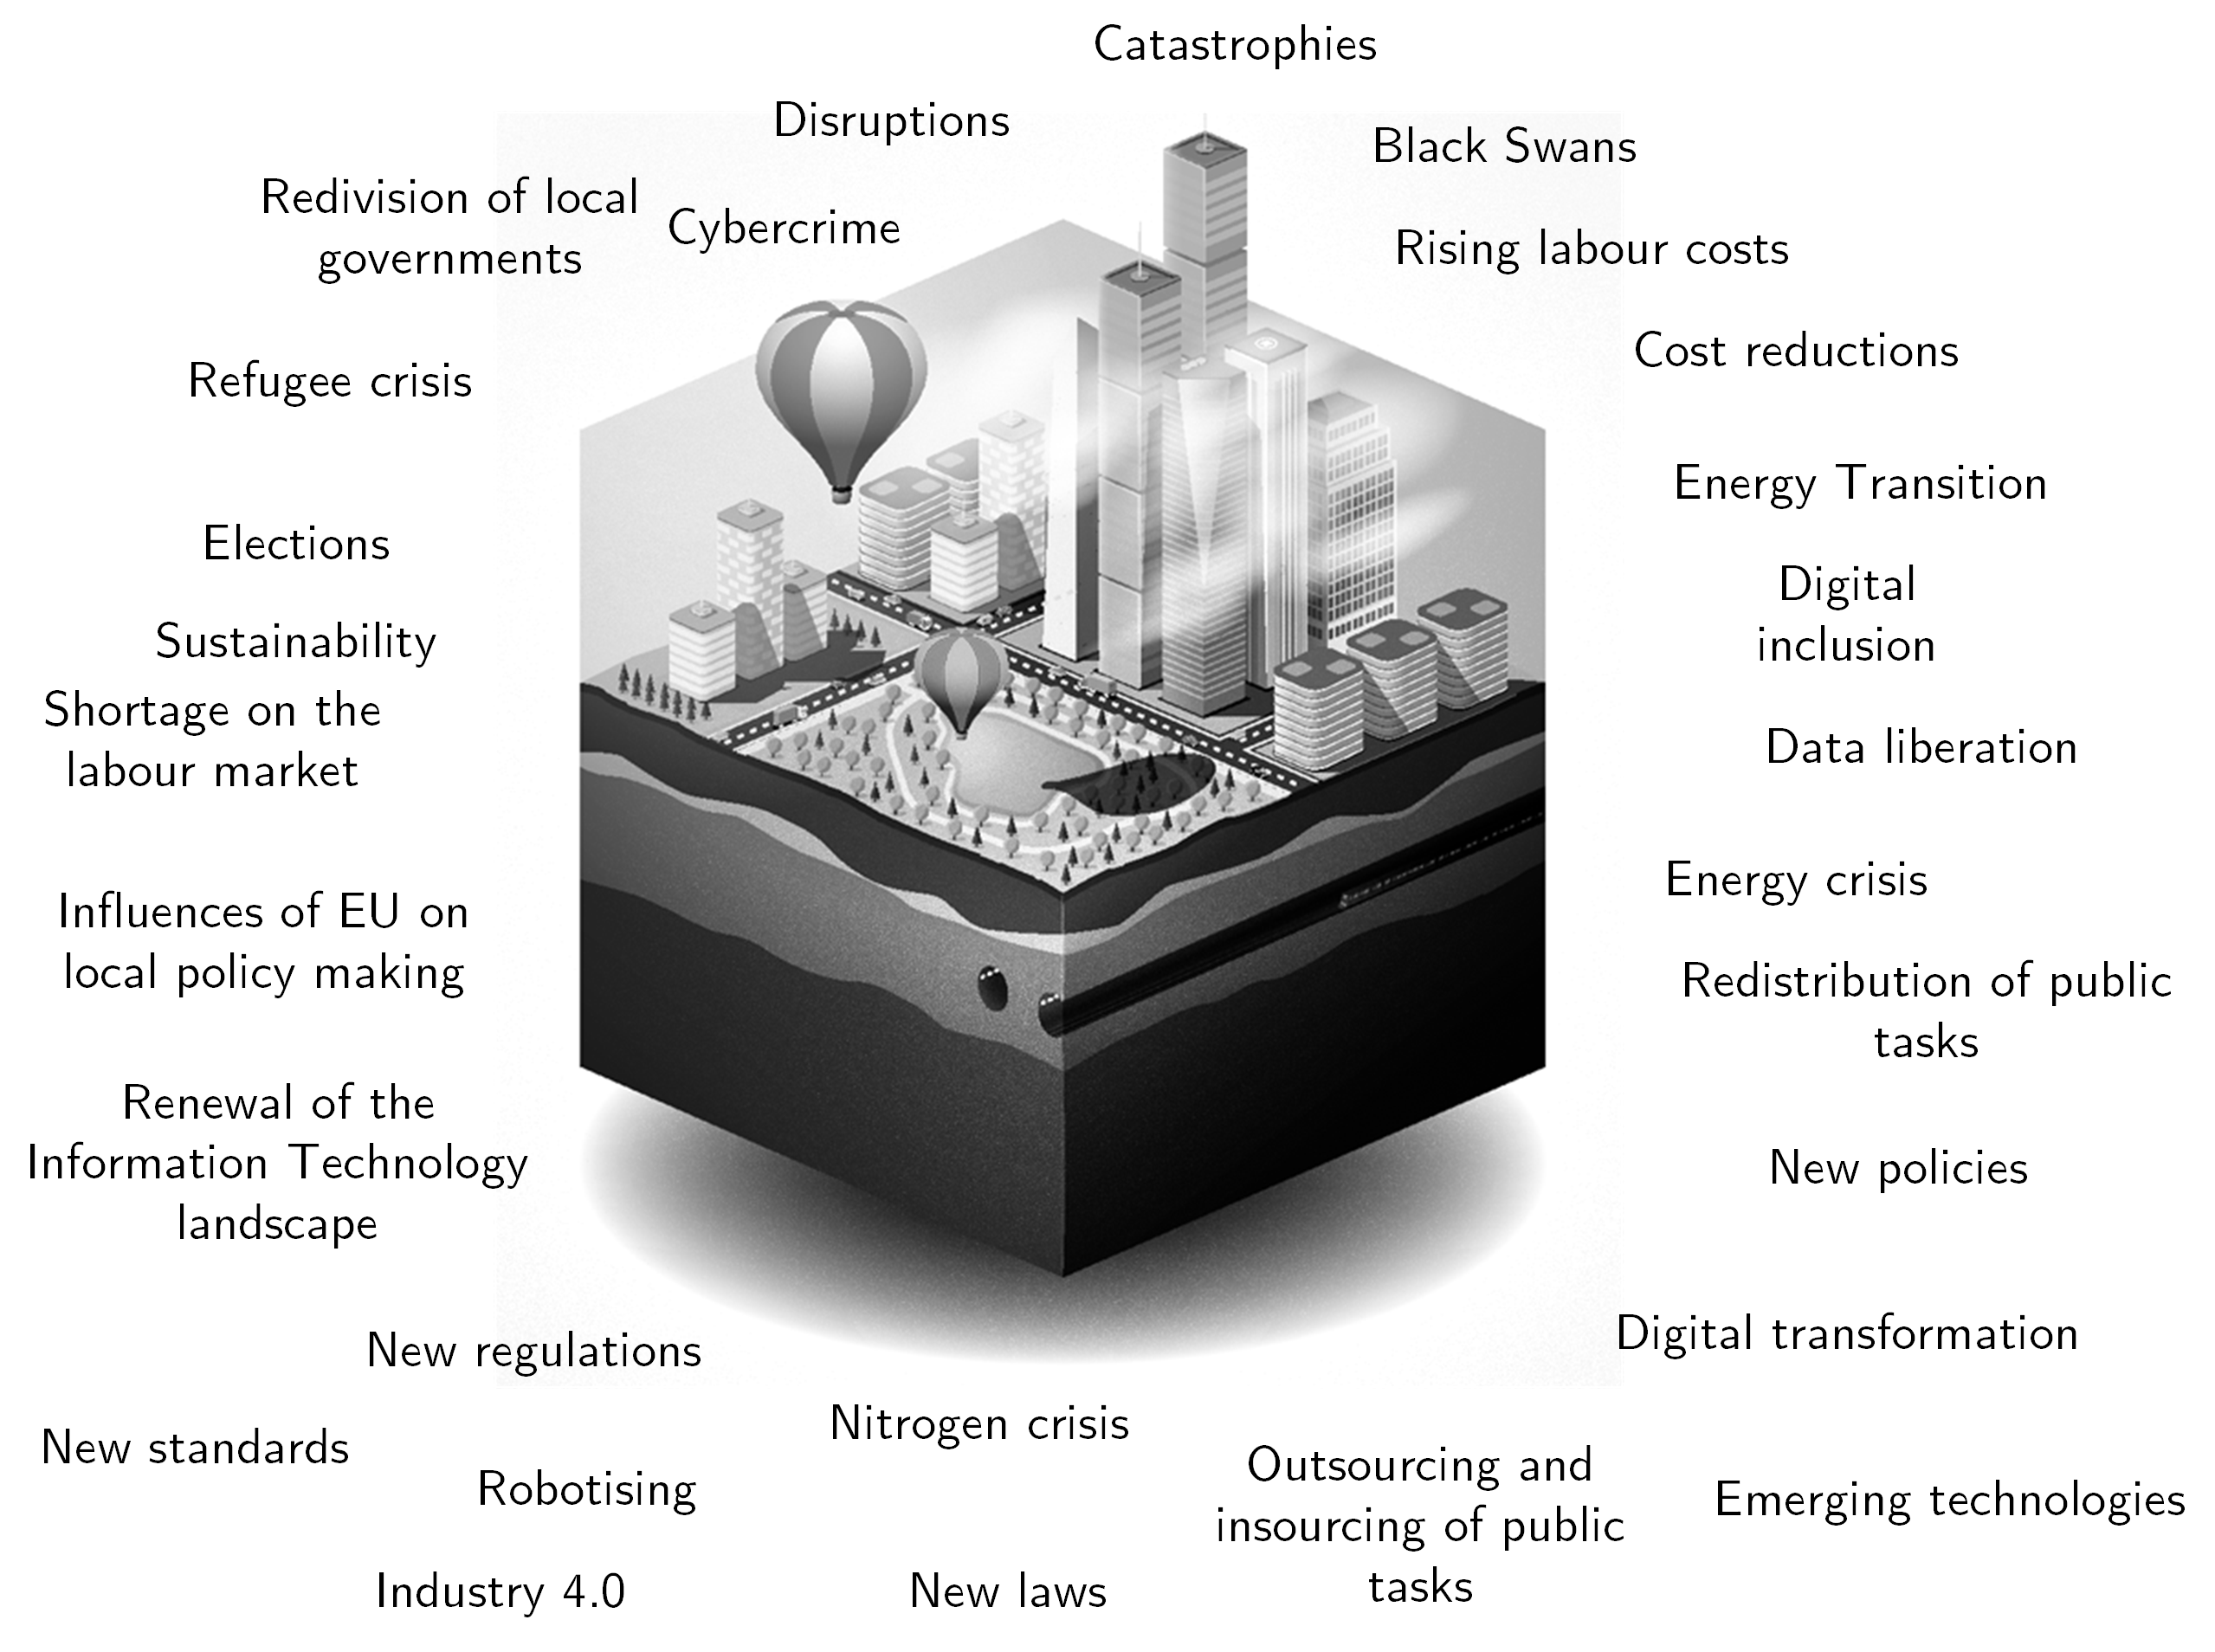
\includegraphics[width=0.8\linewidth]{images/publicstressors}
	\caption[Examples of stressors on the public sector]{Examples of stressors on the public sector}
	\label{fig:publicstressors}
\end{figure}


Because of the \gls{digitaltransformation}, the pace of change is increasing rapidly.  The \gls{digitaltransformation} is not the only stressor on the public sector. There are a lot of internal and external stressors. The public sector invested a lot in being less fragile by becoming more robust and resilient. By being more robust or resilient, you can only withstand the change or the stressor, but you do not gain from it. Governmental agencies in the public sector are searching for methods of dealing with this increased pace and the stressors. The relevance of this research is not only about the addition to the \acrshort{bok} but also to share the outcome with the public sector.

